\chapter{予備知識}
本章では,本研究で開発した個人認証システムで用いた技術について説明する.

% @suppress SectionLength ParagraphNumber JapaneseAmbiguousNounConjunction InvalidSymbol SuccessiveSentence
\section{人工ニューラルネットワーク}
人工ニューラルネットワーク(以下,ニューラルネットワーク)とは,脳内に存在する多数のニューロンによる,シナプスを介した信号のやりとりからなる情報処理の機能を計算機上に再現することを目指したものである.
ニューラルネットワークにおけるニューロンは図\ref{neuron}のように表され,図中の$x_1$から$x_i$からなる入力から,式\ref{calc-neuron}によって$y_j$を出力する.
図\ref{neuron}および式\ref{calc-neuron}においてそれぞれ$w_{j1}$から$w_{ji}$,$w_{ji}$と表されているものはシナプスの結合荷重(以下,結合荷重)で,対応する入力にどれだけの重みを持たせるかを示している.
また,式\ref{calc-neuron}において$b_j$と表されているものはバイアスと呼ばれ,ニューロンが発火する傾向の高さを示している.
式\ref{calc-neuron}における$f$は活性化関数と呼ばれ,入力とそれに対応する結合荷重の積を総和したものにバイアスを足した出力を正規化するために用いる.
活性化関数には恒等写像やReLU(ランプ関数)など様々なものがある.
このようなニューロンを複数個・複数層に重ねることにより,より複雑な問題に対応できる.

\begin{figure}[hbtp]
  \centering
  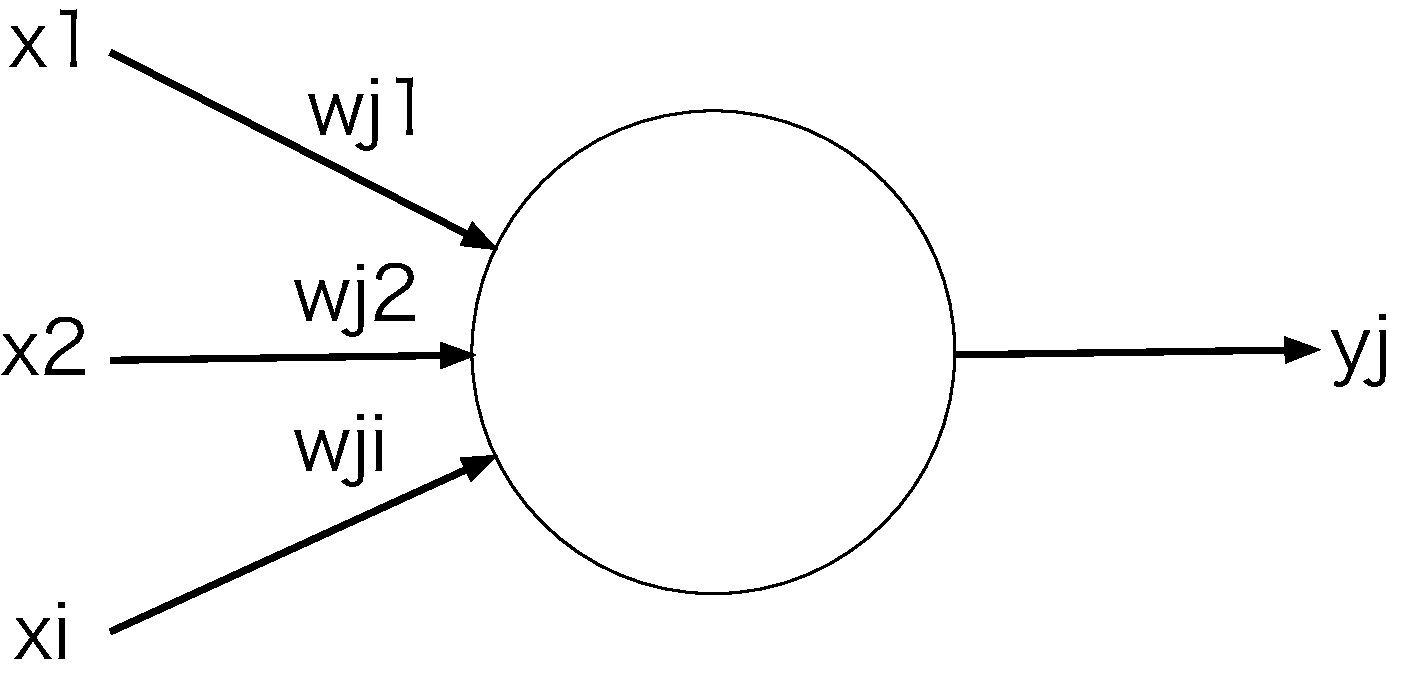
\includegraphics[bb=0 0 683 330, width=8cm]{Figures/neuron.pdf}
  \caption{ニューラルネットワークにおけるニューロン}
  \label{neuron}
\end{figure}

\begin{equation}
\label{calc-neuron}
y_j = f(\sum_i w_{ji} x_i + b_j).
\end{equation}

ただし,ただニューラルネットワークを構築して入力を与えただけでは,期待した出力が得られることは稀である.
そのため,期待した出力が得られるように誤差逆伝播法を用いて結合荷重とバイアスを更新していく,ニューロンの学習を行わなければならない.
学習を行うためには,何を目標に結合荷重やバイアスを更新していくのかという基準を設定する必要がある.
これは損失関数と呼ばれ,ニューラルネットワークにより得られた出力が,期待する出力(以下,教師信号)とどれだけの誤差があるかを定量的に測るために用いられる.

ニューロンの学習を行う際は,図\ref{bp}のような縦軸に損失関数(エネルギー関数)$E$,横軸に結合荷重$w$を置いたグラフで,$E$を最小化するような$opt\_w$に近づくように結合荷重を更新していく(勾配法).

\begin{figure}[hbtp]↲
    \centering↲
    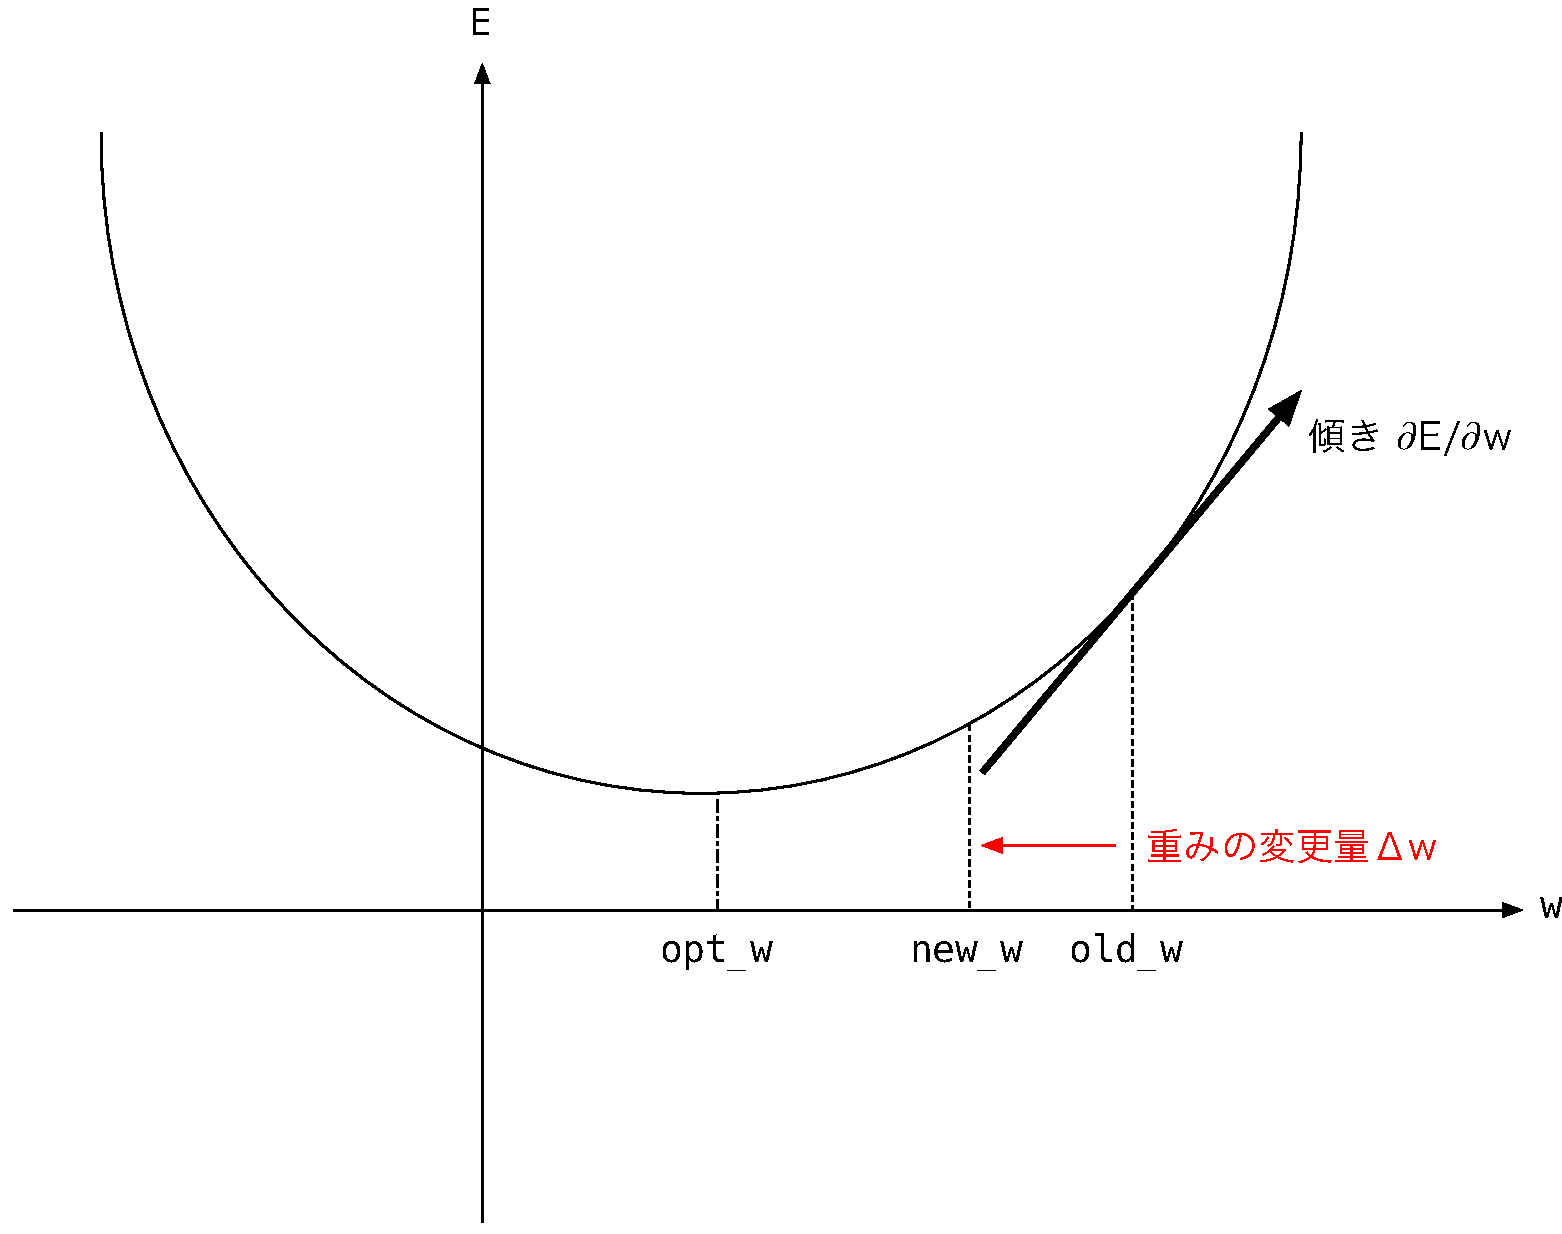
\includegraphics[bb=0 0 749 592, width=9cm]{Figures/bp.pdf}↲
    \caption{ニューロンの結合荷重の更新}↲
    \label{bp}↲
\end{figure}↲

更新した$new\_w$は,式\ref{w-new}で得られる.
\begin{equation}↲
\label{w-new}↲
new\_w = old\_w + \Delta w.↲
\end{equation}↲

式\ref{w-new}における$\Delta w$が結合荷重の変更量となるのだが,これは式\ref{delta-w}で得られる.
\begin{equation}↲
\label{delta-w}↲
\Delta w = - \eta \frac{\partial E}{\partial w}.↲
\end{equation}↲

$\eta$は学習率を表し,どれだけの割合で結合荷重を更新するかを示している.
この値を小さくすることで,結合荷重の更新幅が小さくなる.
その後ろの$\frac{\partial E}{\partial w}$は傾きを示す.↲
結合荷重$w$が$opt\_w$に近づくためには,傾きが正の場合は$\Delta w$が負に,傾きが負の場合は$\Delta w$が正になる必要がある.↲
そのため,$\eta \frac{\partial E}{\partial w}$の結果得られた値の符号を逆にしている.↲

結合荷重の変更量$\Delta w$を得るために必要な傾き$\frac{\partial E}{\partial w}$は,式\ref{ew}で得られる.
\begin{equation}↲
\label{ew}↲
\frac{\partial E_n}{\partial w_{ji}} = \frac{\partial E_n}{\partial a_j} \frac{\partial a_j}{\partial w_{ji}} = \frac{\partial E_n}{\partial a_j} x_i.↲
\end{equation}↲
↲
式\ref{ew}は,合成関数の微分の公式を用いて式変形を行っている.↲
$x_i$は学習中のニューロンに入力された値を示している.↲
ここで,$\frac{\partial E_n}{\partial a_j}$を$\delta_j$と置く.↲
この$\delta_j$と学習中のニューロンの入力値$x_i$を掛けることで傾きが得られ,これに$- \eta$を掛けることで結合荷重の変更量$\Delta w$が得られる.

前述したように,損失関数を用いて教師信号との誤差を測るために用いるのは出力層の出力値である.
ここで,出力層ニューロンの活性化関数と損失関数が特定の組み合わせであれば,$\delta_j$は式\ref{easy-delta}で得られる.
\begin{equation}↲
\label{easy-delta}↲
\delta_j = y_j - t_j.↲
\end{equation}↲

式\ref{easy-delta}における$y_j$は出力層より得られた出力値,$t_j$は教師信号である.
このように極めて単純な計算式で$\delta_j$を得られるため,基本的に出力層では損失関数と活性化関数を合わせて考えるのが一般的である.

まず,ニューラルネットワークで回帰を行う場合は,活性化関数と損失関数にそれぞれ恒等写像(式\ref{identity})と最小二乗誤差(式\ref{lsm})を用いる.
\begin{equation}↲
\label{identity}↲
f(a_j) = a_j.↲
\end{equation}↲
↲
\begin{equation}↲
\label{lsm}↲
E_n = \frac{1}{2} \sum_{k=1}^K (y_{nk} - t_{nk})^2.↲
\end{equation}↲

ニューラルネットワークで二値分類を行う場合は,活性化関数と損失関数にそれぞれシグモイド関数(式\ref{sigmoid})と交差エントロピー誤差(式\ref{ce-1})を用いる.
\begin{equation}↲
\label{sigmoid}↲
f(a_j) = \frac{1}{1 + e^{-a_j}}.↲
\end{equation}↲
↲
\begin{equation}↲
\label{ce-1}↲
E_n = - \sum_{k=1}^K \{t_{nk} \ln y_{nk} + (1 - t_{nk}) \ln (1 - y_{nk)}\}.↲
\end{equation}↲

また,ニューラルネットワークで多クラス分類を行う場合は,活性化関数と損失関数にそれぞれソフトマックス関数(式\ref{softmax})と交差エントロピー誤差(式\ref{ce-2})を用いる.
\begin{equation}↲
\label{softmax}↲
f(a_j) = \frac{e^{a_j}}{\sum_{k=1}^K e^{a_k}}.↲
\end{equation}↲
↲
\begin{equation}↲
\label{ce-2}↲
E_n = - \sum_{k=1}^K t_{nk} \ln y_{nk}.↲
\end{equation}↲

このような組み合わせで出力層を構築することで,前述した式\ref{easy-delta}で$\delta_j$を得られる.

ニューラルネットワークが入力層を含めて3層以上あるような複雑なもので中間層を学習したい場合,この$\delta_j$は式\ref{delta-2}で得られる.
\begin{equation}↲
\label{delta-2}↲
\delta_j = \frac{\partial f}{\partial a_j} \sum_{k=1}^K w_{kj} \delta_k.↲
\end{equation}↲

つまり,学習しているニューロンの活性化関数を微分したものと,出力層に一つ近い層の各結合荷重と$\delta$を掛けたものの総和を掛けることで,中間層の$\delta_j$が得られる.

以上で学習に必要な傾きが得られるが,これを用いた結合荷重の更新方法として式(\ref{w-new})を改良したアルゴリズムが複数考案されている.

まず,確率的勾配降下(SGD)というものがある(式\ref{sgd}).
\begin{equation}↲
\label{sgd}↲
new\_w_{ji} = old\_w_{ji} - \eta \delta_j x_i - \eta \lambda old\_w_{ji}.↲
\end{equation}↲
↲
$- \eta \lambda old\_w_{ji}$は荷重減衰と呼ばれるもので,$\lambda$を正の小さな定数に設定することで傾きがゼロの場合でも結合荷重を減らすことができるというものである.↲
$\eta$の値が結合荷重の更新に強く影響するため,通常は学習の初期段階では大きめの値にし,学習が進むにつれて小さくしていく.↲

次に,AdaGrad\cite{3-adagrad}というものがある(式\ref{adagrad}).↲
\begin{eqnarray}↲
\label{adagrad}↲
new\_g_{ji} = old\_g_{ji} + (\delta_j x_i)^2. \nonumber \\↲
new\_w_{ji} = old\_w_{ji} - \frac{\eta}{\sqrt{new\_g_{ji} + \epsilon}} \delta_j x_i.↲
\end{eqnarray}↲
↲
これは,過去の傾きの二乗和を結合荷重ごとに覚えておき($new\_g_{ji}$),その平方根で$\eta$を割ったものを学習率とする.↲
これにより,総更新量が少ない結合荷重はより大きな幅で,総更新量が多い結合荷重はより小さな幅で更新がなされる.↲
この方式では,学習率が自動的に調整される\cite{3-adagrad-detail}.↲

また,Adam\cite{3-adam}というものがある(式\ref{adam}).
\begin{eqnarray}
\label{adam}
new\_m = \beta_1 old\_m + (1 - \beta_1) \delta_j x_i.\nonumber \\
new\_\nu = \beta_2 old\_\nu + (1 - \beta_2) (\delta_j x_i)^2.\nonumber \\
new\_\hat{m} = \frac{new\_m}{1 - \beta^t_1}.\nonumber \\
new\_\hat{\nu} = \frac{new\_\nu}{1 - \beta^t_2}.\nonumber \\
new\_w_{ji} = old\_w_{ji} - \frac{\alpha}{\sqrt{new\_\hat{\nu}} + \epsilon} new\_\hat{m}.
\end{eqnarray}
↲
まず,傾きの一次モーメント(平均値)と二次モーメント(分散した平方偏差)の概算値を求める($new\_m$及び$new\_\nu$).
そしてこれらの偏りをバイアス補正した推定値を計算することで小さくし($new\_\hat{m}$及び$new\_\hat{\nu}$),これらを用いて結合荷重の更新を行う\cite{3-adam-detail}.

他にも様々なアルゴリズムが提案されている.↲

\section{Autoencoder}
Autoencoderとは,図\ref{autoencoder}のような入力層と出力層のニューロン数を入力データの次元数と同数にし,中間層のニューロン数を一定の割合で削減した3層構造のニューラルネットワークにおいて,入力データと教師信号に同じデータを用いて教師あり学習させたものである.
入力層から中間層への処理をエンコーダ,中間層から出力層への処理をデコーダと呼ぶ.
中間層と出力層の活性化関数は自由に選ぶことができるが,出力層の出力値が教師信号を表現できるような活性化関数を選ばなければならない.

\begin{figure}[hbtp]
  \centering
  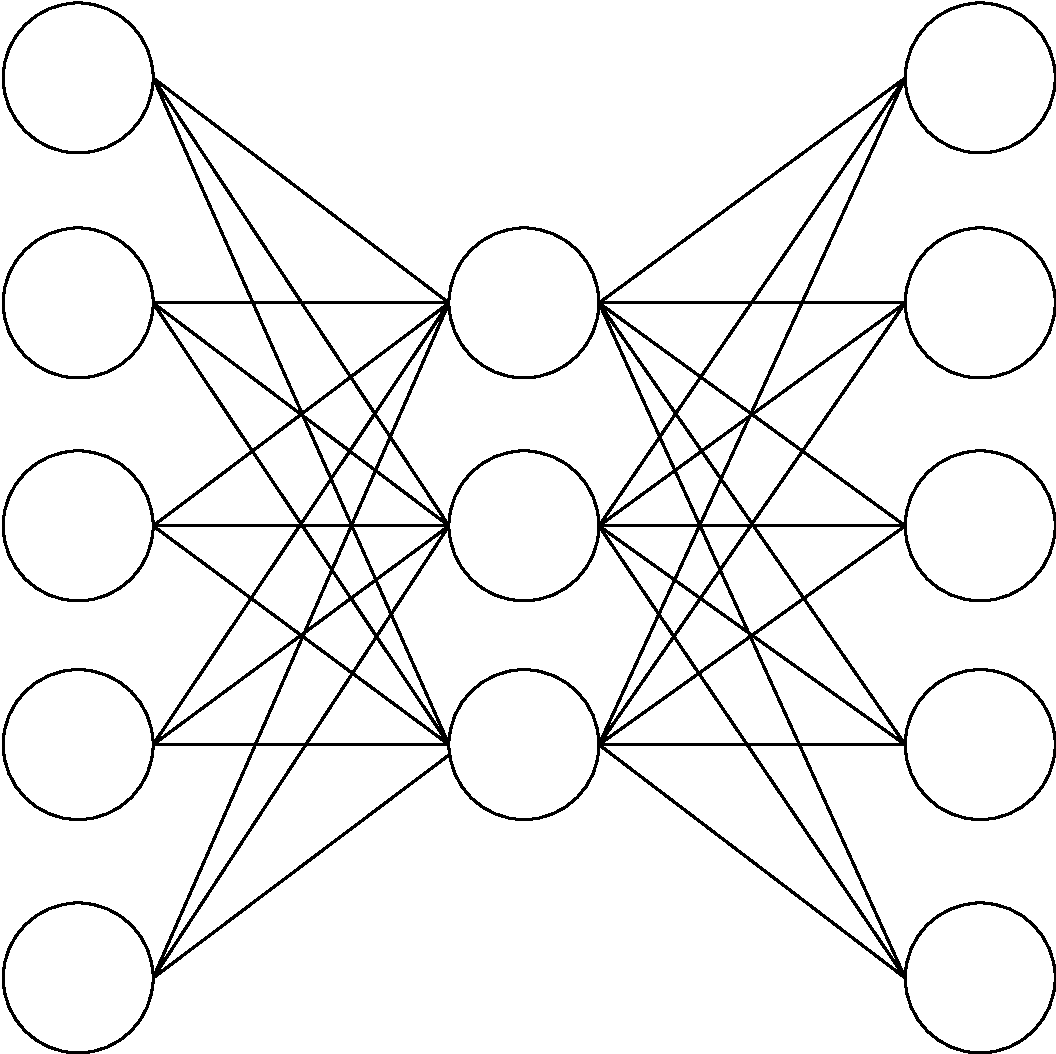
\includegraphics[bb=0 0 507 506, width=8cm]{Figures/autoencoder.pdf}
  \caption{Autoencoder}
  \label{autoencoder}
\end{figure}

Autoencoderの学習を進めた結果出力層の出力と教師信号との誤差が無くなった場合,中間層においてより少ないニューロン数で入力データの情報を表現できていると見ることができる.
このことから,学習済みのAutoencoderからデコーダの部分を取り除き,エンコーダの出力を別のニューラルネットワークへの入力値として渡すことで,入力データの特徴抽出器として用いることができる.

\section{Denoising Autoencoder}
Denoising Autoencoderとは,Autoencoderで用いる入力データに対し一定の割合でランダムなノイズを付与し,ノイズを付与する前の元データを教師信号として与えて教師あり学習させたものである.
入力データにランダムなノイズを付与して学習させることで,入力データの特徴を抽出することに加えてノイズの除去についても学習しなければならなくなり,ノイズに強くより汎化能力の高い特徴抽出器となる.

ノイズの付与方法として,入力データのうちランダムに選択したデータを0にするマスキングノイズや,0か1にする胡麻塩ノイズなど様々なものがある.

\section{Dropout}
Dropoutとは,図\ref{dropout}のように一定の割合でランダムに一部のニューロンを無視して学習を行うものである.
学習後のニューラルネットワークで推定を行う際は,各ニューロンの出力値にDropoutした割合を掛ける.

ニューラルネットワークの学習時にランダムで一部のニューロンを無視することから,複数の独立したニューラルネットワークを学習しているとみなすことができる.
そして推定時にはそれらニューラルネットワークから得られた出力の平均値を求めていると考えられるため,汎化能力がより高くなる.

\begin{figure}[hbtp]
  \centering
  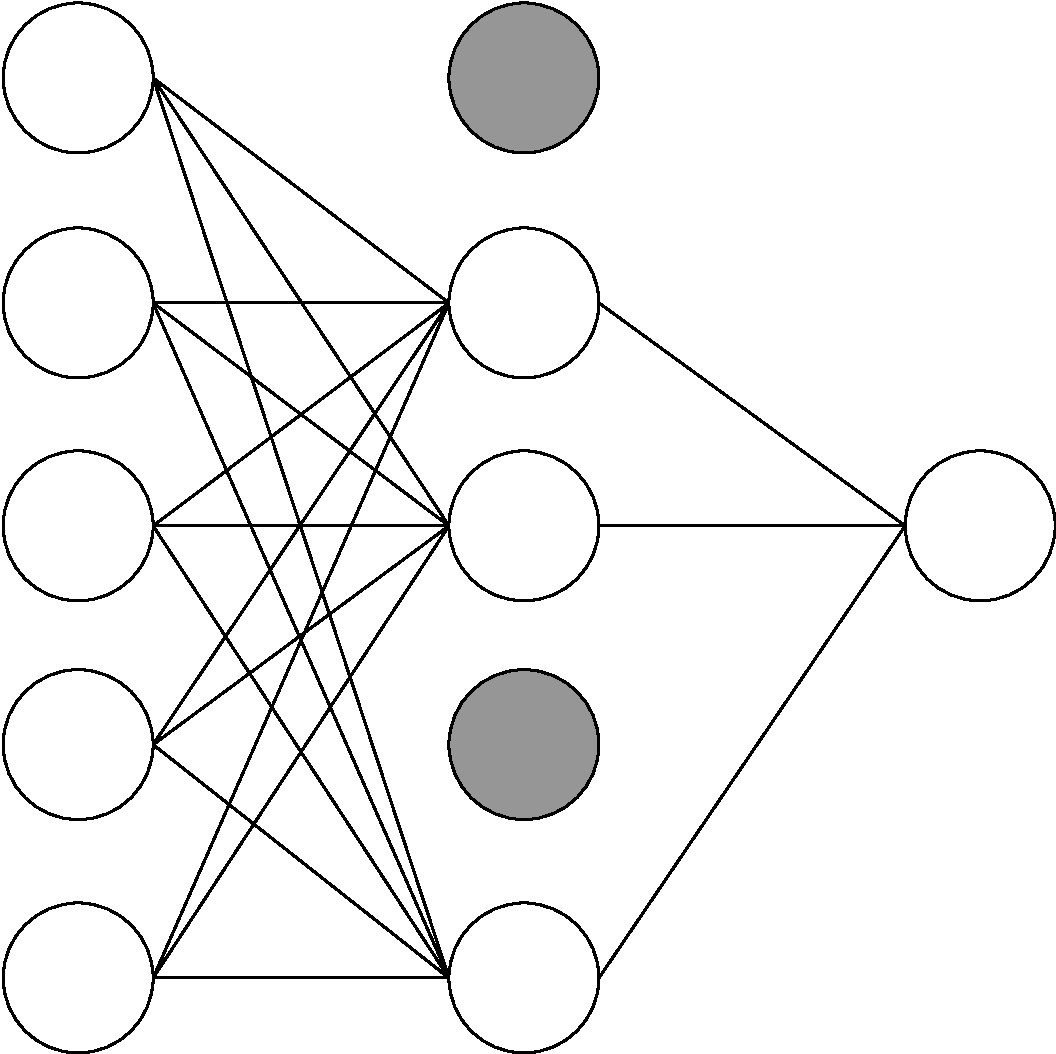
\includegraphics[bb=0 0 507 506, width=8cm]{Figures/dropout.pdf}
  \caption{Dropout}
  \label{dropout}
\end{figure}
